\section{Марериалы работы}

\subsection{Моделирвоание MATLAB}
Соберем схему моделирования двухвассововй системы с заданными параметрами в среде \emph{Matlab Simulink}.
\begin{figure}[!h]
    \centering
    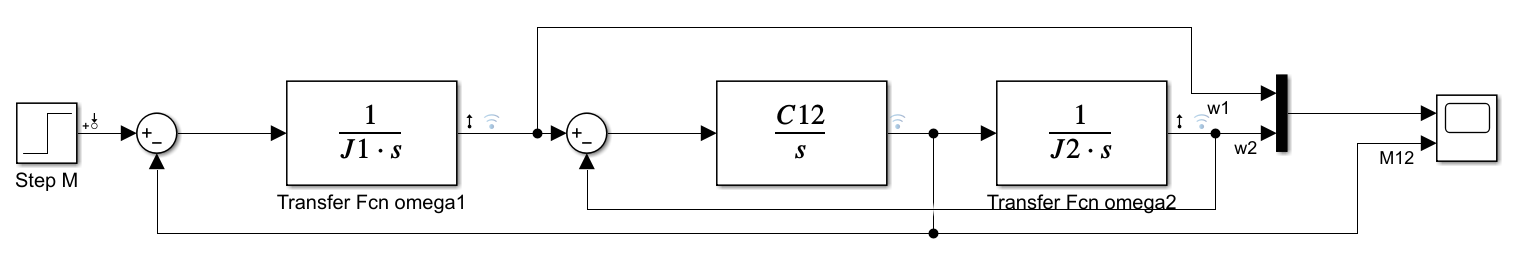
\includegraphics[width=0.9\textwidth]{img/img}
    \caption{Схема моделирования двухмассовой системы}
    \label{fig:dummy}
\end{figure}

Проведем моделирование системы и снимем необходимые графики.
\begin{figure}[!h]
    \centering
    \begin{minipage}{0.5\textwidth}
        \centering
        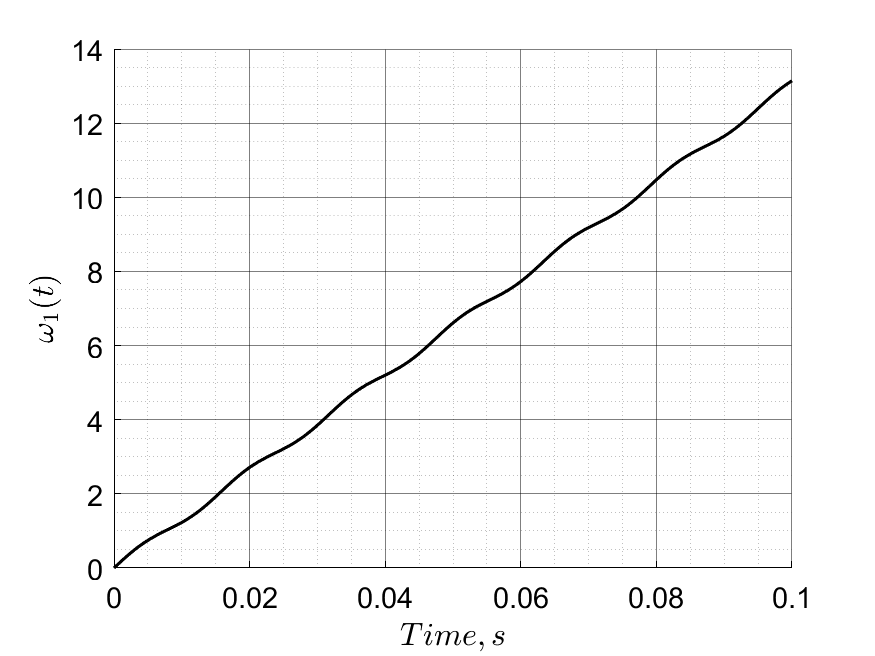
\includegraphics[width = \textwidth]{img/model_omega1}
        \caption{График зависимости $\omega_1(t)$}
%        \label{fig:img/}
    \end{minipage}%
\begin{minipage}{0.5\textwidth}
        \centering
        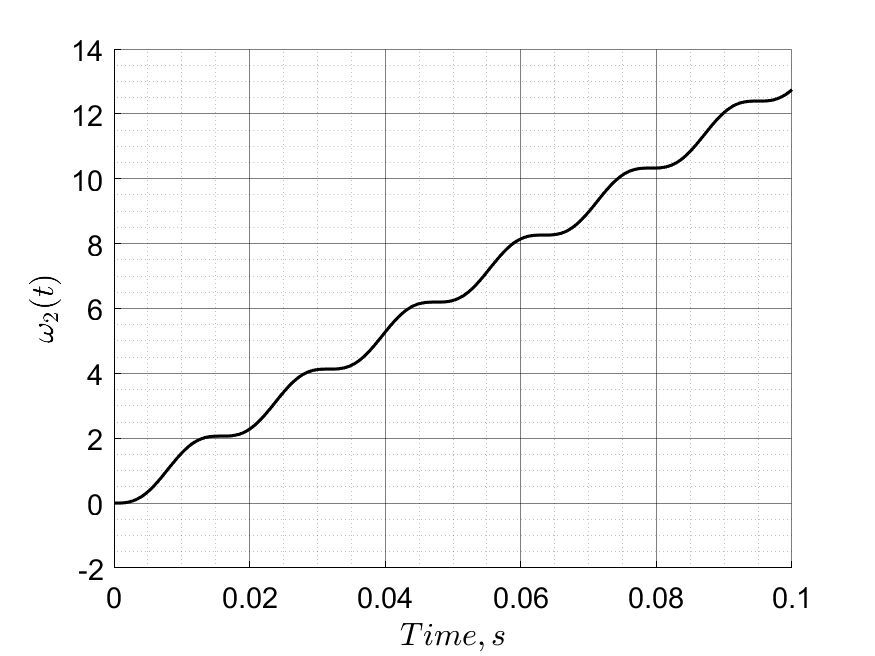
\includegraphics[width = \textwidth]{img/model_omega2}
        \caption{График зависимости $\omega_2(t)$}
%        \label{fig:img/}
    \end{minipage}\label{fig:figure}%
\end{figure}

\begin{figure}[!h]
    \centering
    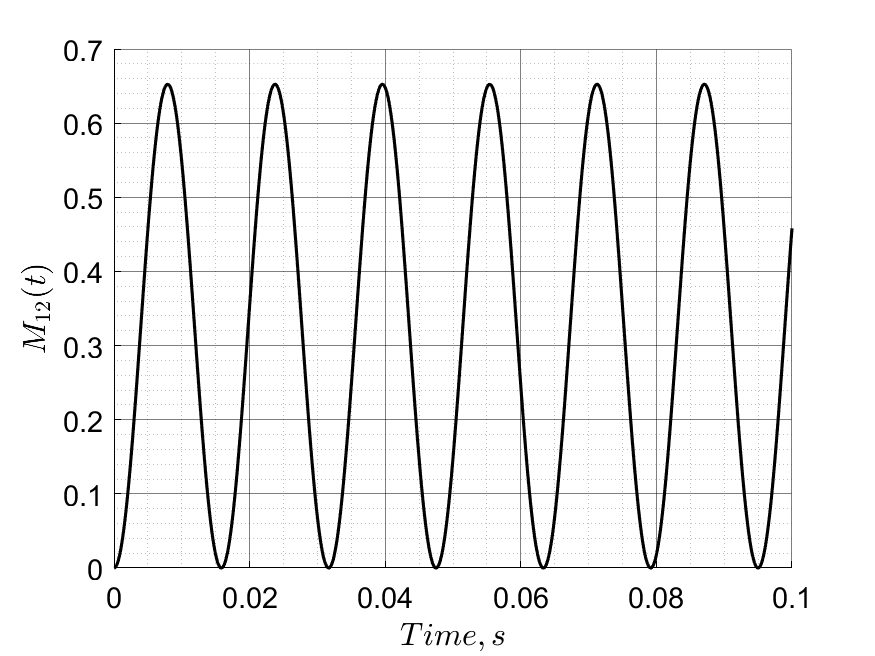
\includegraphics[width=0.5\textwidth]{img/model_M12}
    \caption{График зависимости $M_{12}(t)$}
    \label{fig:model_M12}
\end{figure}

\subsection{Проверка рассчетных параметров}
Для сравнения параметров с расчетными воспользуемся следующими формулами:
\begin{gather*}
    \Omega_0 = \sqrt {\frac{c_{12}(J_1+J_2)}{J_1 J_2}}= 396.8627; \ \ \gamma = \frac{J_1+J_2}{J_1} = 1.3125\\
    \varepsilon_\text{ср} = \frac{M}{J_1+J_2} = 130.4762\\
    \omega_1 = \varepsilon_{\text{ср}} t + \frac{\varepsilon_{\text{ср}}}{\Omega_0}(\gamma-1)\sin(\Omega_0 t) = 130.5t + 0.1027sin(396.9t)\\
    \omega_1 = \varepsilon_{\text{ср}} t -= \frac{\varepsilon_{\text{ср}}}{\Omega_0}\sin(\Omega_0 t) =130.5t - 0.3288sin(396.9t)\\
    M_{12} = J_2\frac{d\omega_2}{dt} = 0.3262 - 0.3262*cos(396.9t)
\end{gather*}

Построим графики полученных величин.
\begin{figure}[!h]
    \centering
    \begin{minipage}{0.5\textwidth}
        \centering
        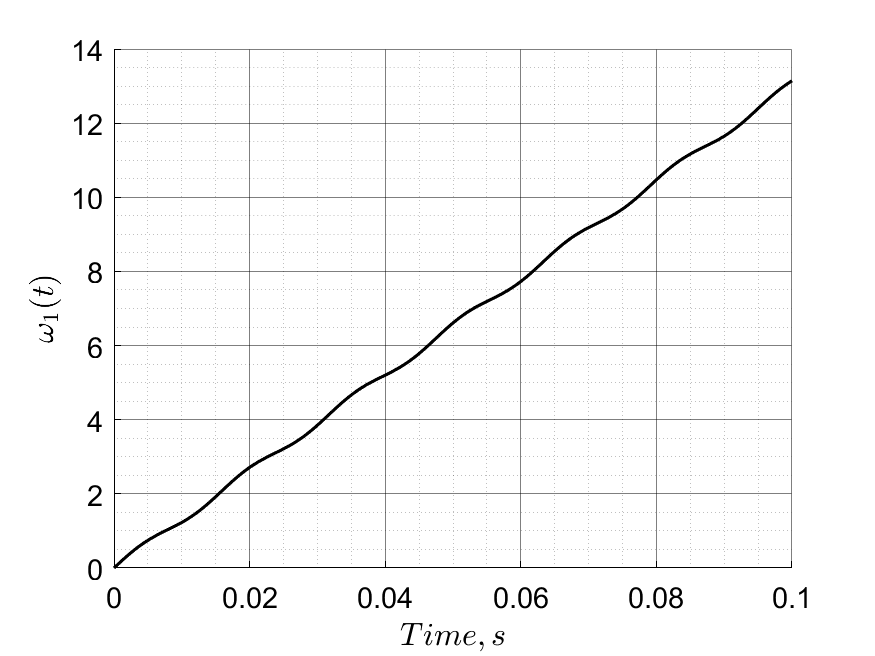
\includegraphics[width = \textwidth]{img/count_omega1}
        \caption{Расчетный график $\omega_1(t)$}
%        \label{fig:img/}
    \end{minipage}%
    \begin{minipage}{0.5\textwidth}
        \centering
        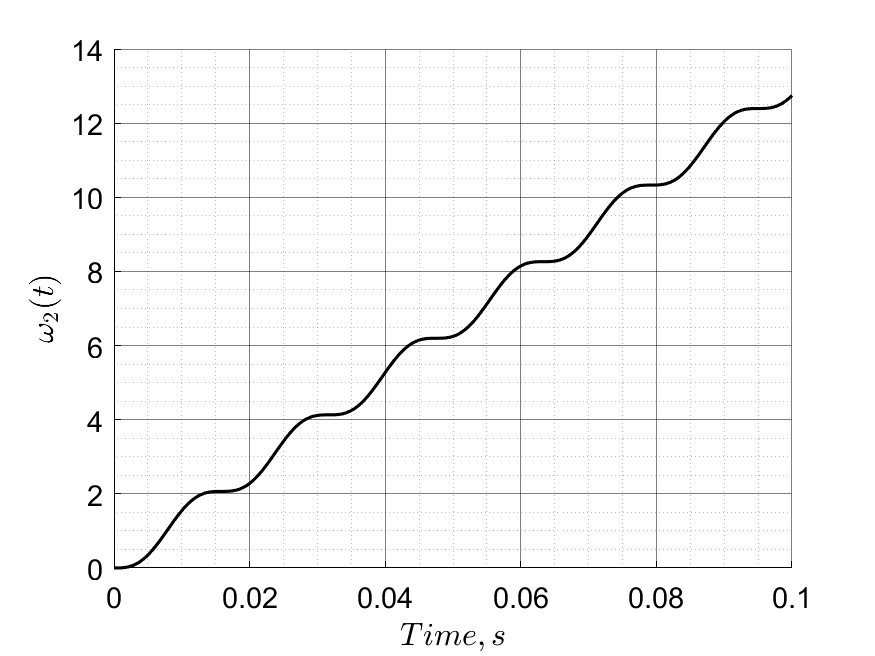
\includegraphics[width = \textwidth]{img/count_omega2}
        \caption{Расчетный график $\omega_2(t)$}
%        \label{fig:img/}
    \end{minipage}\label{fig:figure2}%
\end{figure}

\begin{figure}[!h]
    \centering
    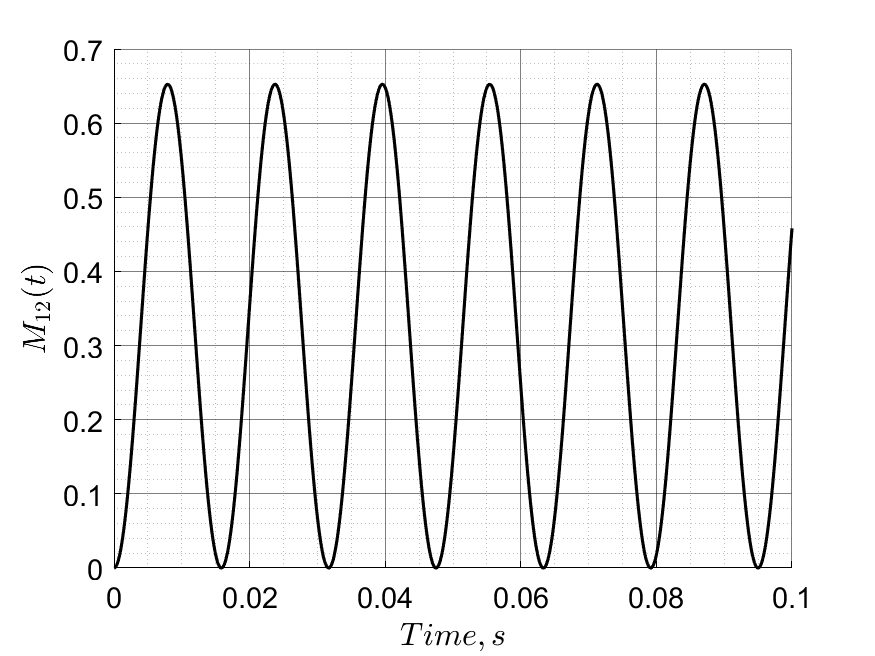
\includegraphics[width=0.5\textwidth]{img/count_M12}
    \caption{Расчетный график $M_{12}(t)$}
    \label{fig:count_M12}
\end{figure}
\newpage
Сравним их на одном графике:
\begin{figure}[!h]
    \centering
    \begin{minipage}{0.5\textwidth}
        \centering
        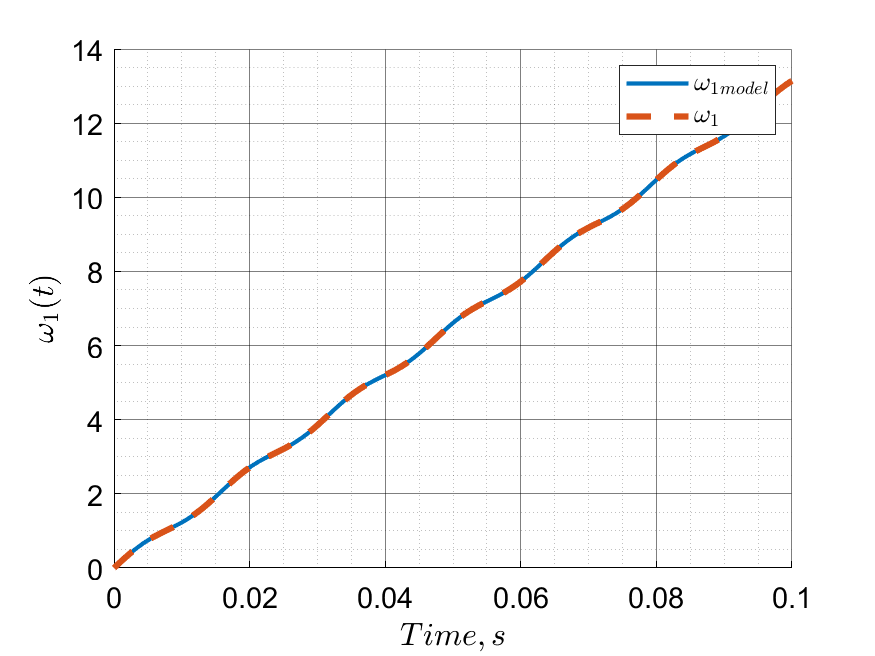
\includegraphics[width = \textwidth]{img/all_omega1}
        \caption{Сравнительный график $\omega_1(t)$}
%        \label{fig:img/}
    \end{minipage}%
    \begin{minipage}{0.5\textwidth}
        \centering
        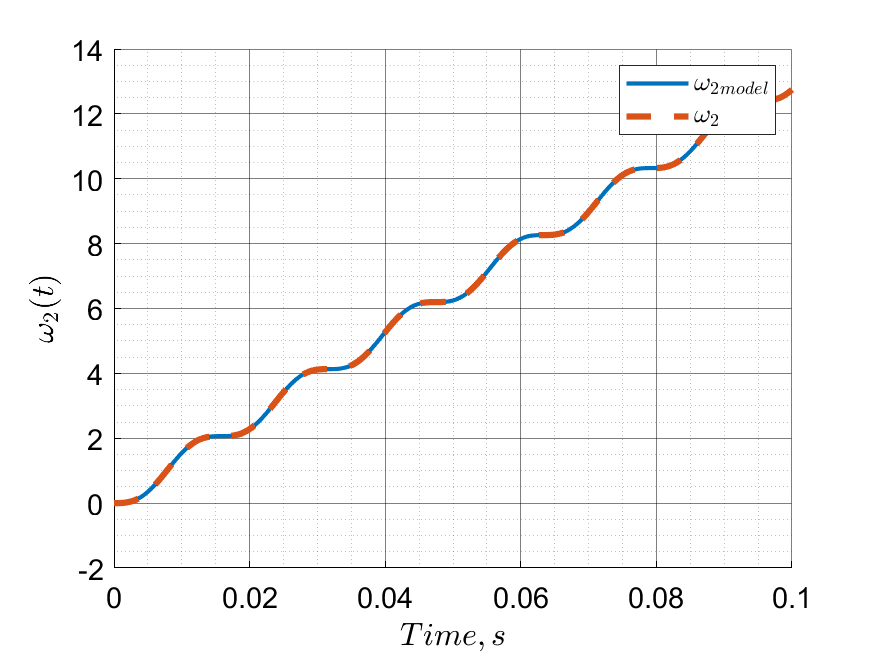
\includegraphics[width = \textwidth]{img/all_omega2}
        \caption{Сравнительный график $\omega_2(t)$}
%        \label{fig:img/}
    \end{minipage}\label{fig:figure4}%
\end{figure}

\begin{figure}[!h]
    \centering
    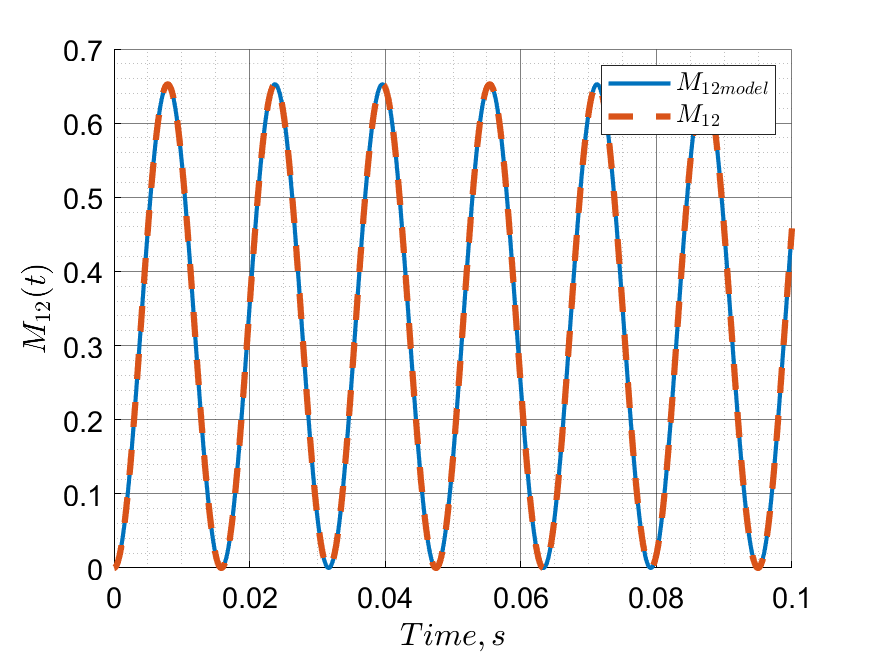
\includegraphics[width=0.5\textwidth]{img/all_M12}
    \caption{Сравнительный график $M_{12}(t)$}
    \label{fig:all_M}
\end{figure}

\newpage
\subsection{Проверка резонансных частот}
\begin{gather*}
    \omega_{c1} = \frac{\Omega_0}{\sqrt{\gamma}} = 346.4102 (\text{рад/c})\\
    \omega_{c2} = \Omega_0= 396.8627 (\text{рад/c})
\end{gather*}

\begin{figure}[!h]
    \centering
    \begin{minipage}{0.5\textwidth}
        \centering
        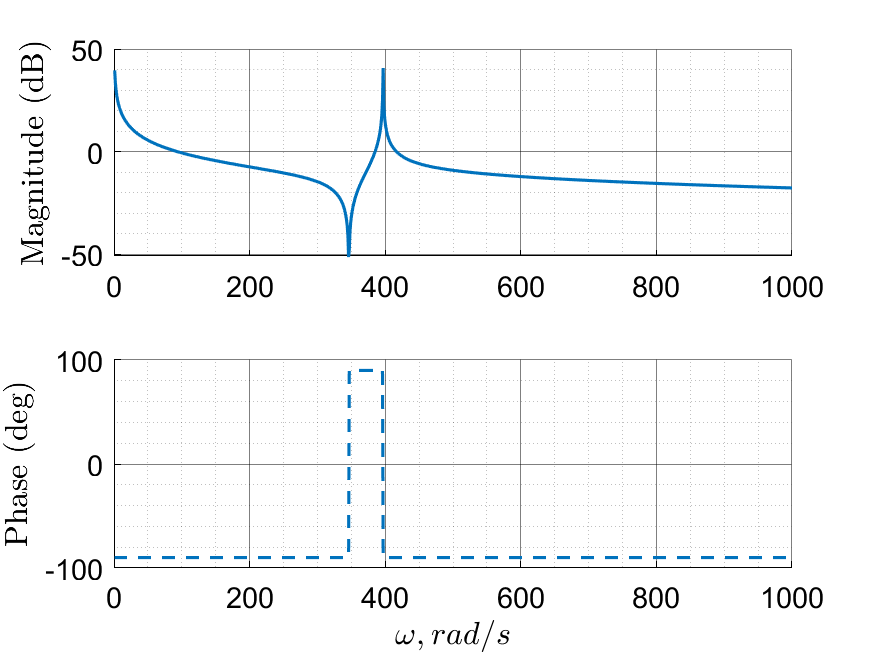
\includegraphics[width = \textwidth]{img/task1_omega1bode}
        \caption{ЛАЧХ и ФЧХ $\omega_1$}
        \label{fig:img/task1_omega1bode}
    \end{minipage}%
\begin{minipage}{0.5\textwidth}
        \centering
        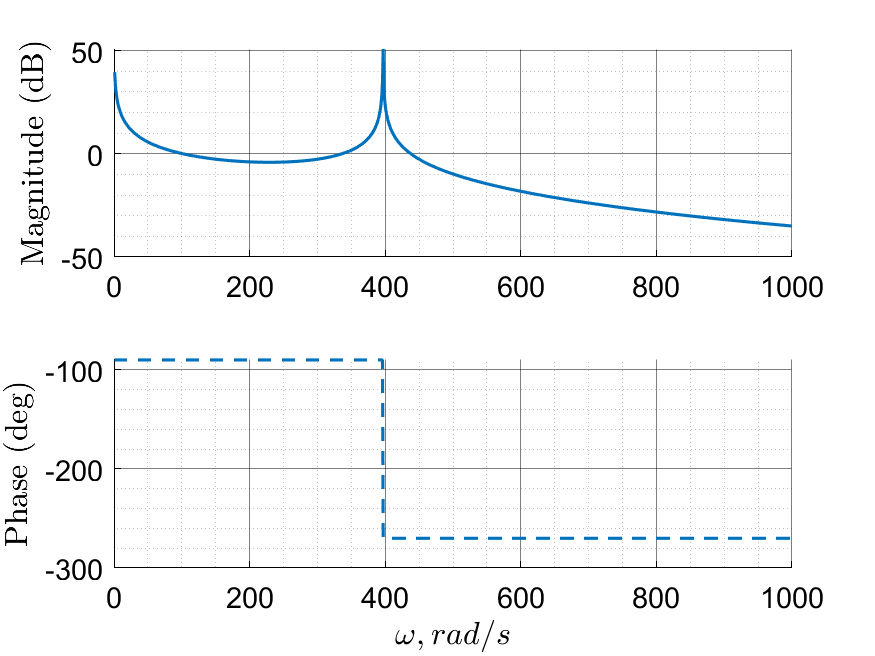
\includegraphics[width = \textwidth]{img/task1_omega2bode}
        \caption{ЛАЧХ и ФЧХ $\omega_2$}
        \label{fig:img/task1_omega2bode}
    \end{minipage}%
\end{figure}




